%% Le lingue utilizzate, che verranno passate come opzioni al pacchetto babel. Come sempre, l'ultima indicata sarà quella primaria.
%% Se si utilizzano una o più lingue diverse da "italian" o "english", leggere le istruzioni in fondo.
\def\thudbabelopt{english,italian}
%% Valori ammessi per target: bach (tesi triennale), mst (tesi magistrale), phd (tesi di dottorato).
%% Valori ammessi  per aauheader: '' (vuoto -> nessun header Alpen Adria Univeristat), aics (Department of Artificial Intelligence and Cybersecurity), informatics (Department of Informatics Systems). Il nome del dipartimento è allineato con la versione inglese del logo UniUD.
%% Valori ammessi per style: '' (vuoto -> stile moderno), old (stile tradizionale).
\documentclass[target=bach,aauheader=,style=]{thud}

%% --- Informazioni sulla tesi ---
%% Per tutti i tipi di tesi
% Scommentare quello di interesse, o mettete quello che vi pare
\course{Informatica}
%\course{Internet of Things, Big Data e Web}
%\course{Matematica}
%\course{Comunicazione Multimediale e Tecnologie dell'Informazione}
\title{Implementazione in Erlang dell'algoritmo GHS per il calcolo di un Albero Minimo di Copertura}
\author{Riccardo Cavasin}
\supervisor{Prof.\ Gabriele Puppis}
% \cosupervisor{?}
% \tutor{Guido Necchi}
%% Campi obbligatori: \title, \author e \course.
%% Altri campi disponibili: \reviewer, \tutor, \chair, \date (anno accademico, calcolato in automatico), \rights
%% Con \supervisor, \cosupervisor, \reviewer e \tutor si possono indicare più nomi separati da \and.
%% Per le sole tesi di dottorato:
% \phdnumber{313}
% \cycle{XXVIII}
% \contacts{Via della Sintassi Astratta, 0/1\\65536 Gigatera --- Italia\\+39 0123 456789\\\texttt{http://www.example.com}\\\texttt{inbox@example.com}}

%% --- Pacchetti consigliati ---
%% pdfx: per generare il PDF/A per l'archiviazione. Necessario solo per la versione finale
\usepackage[a-1b]{pdfx}
%% hyperref: Regola le impostazioni della creazione del PDF... più tante altre cose. Ricordarsi di usare l'opzione pdfa.
\usepackage[pdfa]{hyperref}
%% tocbibind: Inserisce nell'indice anche la lista delle figure, la bibliografia, ecc.

%% --- Stili di pagina disponibili (comando \pagestyle) ---
%% sfbig (predefinito): Apertura delle parti e dei capitoli col numero grande; titoli delle parti e dei capitoli e intestazioni di pagina in sans serif.
%% big: Come "sfbig", solo serif.
%% plain: Apertura delle parti e dei capitoli tradizionali di LaTeX; intestazioni di pagina come "big".

\usepackage[disable]{todonotes}
\usepackage{amsmath}
\usepackage{amsthm}
\usepackage{amssymb}
\usepackage{textcomp}
\usepackage{xcolor}
\usepackage{colorprofiles}
\usepackage{listings}
\usepackage{xparse}
\usepackage{graphicx}
\usepackage{float}
\usepackage{tikz}
\usetikzlibrary{positioning,chains,fit,shapes,calc,arrows,patterns,external,shapes.callouts,graphs,matrix}
\renewcommand{\restriction}{\mathord{\upharpoonright}}
\newcommand{\eng}[1]{\foreignlanguage{english}{#1}}
\makeatletter
    \@ifdefinable{\selected}{\def\selected/{\eng{selected}}}
    \@ifdefinable{\rejected}{\def\rejected/{\eng{rejected}}}
    \@ifdefinable{\undecided}{\def\undecided/{\eng{undecided}}}
\makeatother
\newcommand{\sub}[1]{$_#1$}
\NewDocumentCommand{\msg}{m o}{\textlangle\lstinline{#1}\IfNoValueF{#2}{, #2}\textrangle}
\newtheorem{lemma}{Lemma}
\newtheorem{corollary}{Corollario}[lemma]
\newtheorem*{exmp}{Esempio}
\setlength{\marginparwidth}{2cm}
\definecolor{codegreen}{rgb}{0,0.6,0}
\definecolor{codegray}{rgb}{0.5,0.5,0.5}
\definecolor{codepurple}{rgb}{0.58,0,0.82}
\definecolor{backcolour}{rgb}{0.95,0.95,0.92}

\lstdefinestyle{teletype}{
    backgroundcolor=\color{backcolour},
    commentstyle=\color{codegreen},
    keywordstyle=\color{magenta},
    numberstyle=\tiny\color{codegray},
    stringstyle=\color{codepurple},
    basicstyle=\ttfamily\footnotesize,
    breakatwhitespace=false,         
    breaklines=true,                 
    captionpos=b,                    
    keepspaces=true,                 
    numbers=left,                    
    numbersep=5pt,                  
    showspaces=false,                
    showstringspaces=false,
    showtabs=false,                  
    tabsize=2
}
\lstset{style=teletype}

\usetikzlibrary{nfold}
\makeatletter
\tikzset{
  side by side/.style args={#1:#2}{
    postaction={path only,draw=#1,offset=+.5\pgflinewidth},
    postaction={path only,draw=#2,offset=+-.5\pgflinewidth}},
  side by side'/.style={path only,side by side={#1}},
  offset/.code=
    \tikz@addoption{%
      \pgfgetpath\tikz@temp
      \pgfsetpath\pgfutil@empty
      \pgfoffsetpath\tikz@temp{#1}}}
\makeatother

\begin{document}
\maketitle
%% Dedica (opzionale)
% \begin{dedication}
% 	Al mio gatto,\par per essere rotondo.
% \end{dedication}

%% Ringraziamenti (opzionali)
% \acknowledgements
% Grazie ad alvise bruniera per avermi controllato la tesi

%% Sommario (opzionale)
\abstract

L'algoritmo di Gallager-Humblet-Spira (denominato GHS) è un algoritmo distribuito per il calcolo di un \eng{Minimum Spanning Tree} (MST) in una rete di calcolatori. Gli MST hanno varie applicazioni nei sistemi distribuiti, come per esempio la costruzione di alberi di \eng{broadcast} efficienti o il calcolo dei cammini minimax/\eng{widest path}.

In questa tesi si presenta un'implementazione dell'algoritmo in linguaggio Erlang, e una sua applicazione per il calcolo distribuito dei cammini minimax. Si esamina in dettaglio l'algoritmo e si presentano le caratteristiche della programmazione distribuita in generale, tra cui il problema del leader \eng{election}, il problema del \eng{reliable broadcast} e le misure di complessità degli algoritmi distribuiti in termini di numero di messaggi, tempo e spazio.

Si presentano inoltre il modello ad attori, su cui si basa Erlang, e l'architettura di ERTS, in particolare la macchina virtuale BEAM, lo scheduler e il sistema di scambio di messaggi.

Infine, si discutono le scelte implementative: il metodo di generazione degli \eng{input}, la validazione dei risultati e la struttura del progetto.

\listoftodos

%% Indice
\tableofcontents

%% Lista delle tabelle (se presenti)
%\listoftables

%% Lista delle figure (se presenti)
% \listoffigures

%% Corpo principale del documento
\mainmatter

\chapter{Introduzione}

In questa tesi si presenta un'implementazione in linguaggio Erlang dell'algoritmo distribuito di Gallager-Humblet-Spira~\cite{10.1145/357195.357200} (denominato GHS) per il calcolo di un albero minimo di copertura (\eng{Minimum Spanning Tree}~\textendash\,~MST). In un grafo non orientato, connesso e pesato, uno \eng{spanning tree} è un sottografo connesso aciclico \,\textendash\,~un \emph{albero}~\,\textendash\, che connette tutti i nodi. Un MST è uno \eng{spanning tree} tale che la somma dei pesi degli archi è minima, e in un grafo possono esistere più MST. L'algoritmo GHS supporta anche grafi non connessi, in tal caso si ottiene un MST per ogni componente connessa.
\bigskip

Gli algoritmi tradizionali per il calcolo dell'MST, come ad esempio Kruskal o Prim, non sono generalmente applicabili ai contesti distribuiti. Gli algoritmi distribuiti sono progettati per essere eseguiti simultaneamente da più elaboratori interconnessi. Non è detto che esista un elaboratore con una visione completa della rete, l'algoritmo deve svolgersi in maniera cooperativa. Inoltre, la dimensione della rete potrebbe essere tale da non poter essere rappresentata completamente nella memoria di un singolo elaboratore.

Le reti sono modellate come grafi non orientati dove i nodi rappresentano gli elaboratori e gli archi le connessioni; si può inoltre scegliere una metrica delle connessioni \,\textendash\,~come ad esempio la larghezza di banda, la latenza, ecc~\,\textendash\, e rappresentarla come costo degli archi. Sulle reti dei sistemi distribuiti trovano applicazioni pratiche molti problemi tipici dei grafi, ma la loro implementazione in forma distribuita non è sempre triviale. Gli MST hanno svariate applicazioni nei sistemi distribuiti; a titolo di esempio menzioniamo il problema del cammino minimax, che sarà utilizzato per dimostrare la nostra implementazione dell'algoritmo.

I sistemi distribuiti presentano anche classi di problemi più generali: verranno esaminati in particolare il problema del \emph{\eng{leader election}} e il problema del \emph{\eng{reliable broadcast}}, poiché sono risolti dall'algoritmo GHS.

In questa tesi ci focalizzeremo sul caso in cui la topologia del grafo è statica, ogni nodo è identificato da un id univoco e le connessioni sono senza errori e FIFO.
\bigskip

Il carattere concorrente dei sistemi distribuiti può essere modellato con il formalismo di calcolo ``ad attori''. Un attore è l'unità di base in una computazione concorrente, possiede uno stato proprio e comunica con altri attori inviando e ricevendo messaggi in modo asincrono. La comunicazione avviene esclusivamente tra coppie di nodi mediante l'utilizzo di indirizzi univoci. Un attore può creare un altro attore e ottenerne l'indirizzo, oppure può riceve l'indirizzo di altri attori via messaggio.  Il punto principale del modello ad attori è l'assenza di risorse condivise e quindi situazioni di contesa che necessiterebbero sincronizzazione; tuttavia situazioni di \eng{deadlock} possono comunque verificarsi nel caso di attese cicliche di messaggi.

Il linguaggio Erlang in cui è implementato l'algoritmo è un linguaggio orientato allo sviluppo di sistemi distribuiti basato sul modello ad attori. Un attore è rappresentato come un processo isolato, la cui creazione e distruzione è un'operazione a basso costo. I processi sono identificati da un PID e possono interagire solamente mediante scambio di messaggi, in maniera trasparente anche tra nodi Erlang su macchine diverse. I messaggi sono distribuiti attraverso canali affidabili FIFO a destinatari noti.
\bigskip

I sorgenti dell'implementazione sono disponibili su una \href{https://github.com/Lucide/Gallager-Humblet-Spira}{\eng{repository}} git pubblica.

\chapter{L'algoritmo GHS}

\section{Cenni sugli MST}

Un grafo non orientato connesso e pesato $G$ è una tupla $\langle V,E,w\rangle$ dove $V$ è l'insieme dei nodi, $E$ è l'insieme degli archi intesi come coppie non ordinate di nodi e $w\colon E\to\mathbb{R}$ è una funzione che associa un peso a ogni arco. Si indica la dimensione del grafo con $|G|$, dove $|G|=|V|$. Viene anche definito il peso di $G$ come:
$$
W(G)=\sum_{e\in E}w(e)
$$
Uno \eng{spanning tree} è un sottografo $G'$ di $G$ tale che:
\begin{enumerate}
  \item $G'=\langle V,E',w\restriction_{E'}\rangle$, dove $E'\subseteq E$
  \item $G'$ è connesso
  \item $G'$ è aciclico
\end{enumerate}
Un grafo non orientato connesso e aciclico è chiamato un albero.
\begin{lemma}\label{mst:path}
In un albero, ogni coppia di nodi è connessa da uno e uno solo cammino.
\end{lemma}
\begin{proof}
Se per assurdo non esistesse, il grafo non sarebbe connesso e quindi non sarebbe un albero, assurdo. Altrimenti, se per assurdo esistesse più di un cammino, la loro unione conterrebbe almeno un ciclo e quindi il grafo non sarebbe un albero, assurdo.
\end{proof}
Uno \eng{spanning tree} $G'$ è un \eng{\emph{minimum} spanning tree} se $W(G')\leq W(G'')$ per ogni \eng{spanning tree} $G''$. In generale, l'MST non è unico:
\begin{exmp}
Dato un grafo completo di tre nodi $G=\langle\{a,b,c\},\{e_1,e_2,e_3\},w\rangle$, dove $w(e_1)=w(e_2)\:>w(e_3)$. Un MST sarà costituito dagli archi $\{e_1, e_3\}$, l'altro da $\{e_1, e_3\}$. Definiamo \emph{frammento} un sottografo connesso di un qualche MST.
\begin{figure}[H]
    \centering
    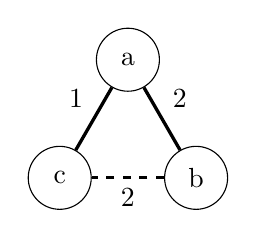
\begin{tikzpicture}
        \graph [clockwise=3,radius=1cm,nodes={circle, minimum size=0.8cm, draw}] {
            a/a,
            b/b,
            c/c,
        };
        \graph {
        (a) -- [edge label=$2$, very thick] (b),
        (b) -- [edge label=$2$, very thick, dashed] (c),
        (c) -- [edge label=$1$, very thick] (a),
        };
    \end{tikzpicture}
    \hspace{2cm}
    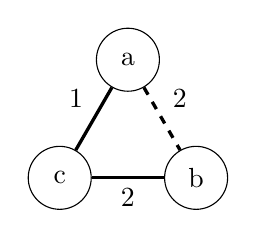
\begin{tikzpicture}
        \graph [clockwise=3,radius=1cm,nodes={circle, minimum size=0.8cm, draw}] {
            a/a,
            b/b,
            c/c,
        };
        \graph {
        (a) -- [edge label=$2$, very thick, dashed] (b),
        (b) -- [edge label=$2$, very thick] (c),
        (c) -- [edge label=$1$, very thick] (a),
        };
    \end{tikzpicture}
    \caption{Due possibili MST dello stesso grafo.}
\end{figure}
\end{exmp}
\begin{lemma}[Unicità degli MST]\label{mst:uniqueness}
Se esiste più di un MST, allora esistono due archi $e_1,e_2\;\in E$ con lo stesso peso.
\end{lemma}
\begin{proof}
Supponiamo per assurdo che esistano due MST di $G$ diversi $H=\langle V,E_H,w\rangle$, $S=\langle V,E_S,w\rangle$, e che tutti gli archi abbiano peso distinto. Allora esiste un unico arco $e_1$ di peso minimo tale che $e_1\in E_H\land e_1\notin E_S\;$ o $\;e_1\in E_S\land e_1\notin E_H$. Senza perdita di generalità, assumiamo $e_1\in E_H$. $S$ è un albero di copertura, quindi aggiungendo l'arco $e_1$ a $S$, si crea un ciclo. A sua volta, $H$ è un albero, quindi è aciclico ed esiste un arco $e_2$ nel ciclo tale $e_2\in E_S\;\land\;e_2\notin E_H$. Per ipotesi, $w(e_1)<w(e_2)$, poiché $e_1$ è stato scelto come minimo. $e_1$ e $e_2$ fanno entrambi parte del ciclo, quindi sostituendo $e_1$ a $e_2$ in $S$ si ottiene uno \eng{spanning tree} diverso di peso minore. Ma allora $S$ non era un MST, assurdo.
\end{proof}
\begin{corollary}
Se tutti gli archi hanno peso distinto, l'MST è unico.
\end{corollary}

\begin{lemma}[Proprietà del taglio]\label{mst:cut}
Un taglio di un grafo è un partizionamento $C=(S,V\setminus S)$, $S\subseteq V$ di $V$ in due parti. Un arco $(u,v)\in E$, $u,v\in V$ si dice di attraversamento se $u\in S\;\land\;v\in V\setminus S$ oppure $v\in S\;\land\;u\in V\setminus S$.\\
Per ogni taglio $C$ nel grafo, se l'arco di attraversamento di peso minimo è unico, allora appartiene a tutti gli MST.
\end{lemma}
\begin{proof}
Supponiamo per assurdo che esista un MST $H$ che non contiene l'arco di attraversamento minimo $e$. $H$ è un albero di copertura, quindi aggiungendo l'arco $e$ a $H$ si ottiene un ciclo che attraversa il taglio in $e$ e $e'$. Per ipotesi, $w(e)<w(e')$, poiché $e'$ è stato scelto come minimo. Sostituendo $e'$ a $e$ in $H$ si ottiene uno \eng{spanning tree} di peso minore ad $H$. Ma allora $H$ non era un MST, assurdo.
\end{proof}
\begin{corollary}
Come corollario, nel caso generale, gli archi di attraversamento di peso minimo appartengono ciascuno a un qualche MST. Questi archi si dicono \emph{\eng{safe}}.
\end{corollary}

Si nota che il problema del \eng{minimum spanning tree}, a differenza del problema dei cammini mimi, è ben definito anche in caso di cicli di peso negativo.
Nel caso $G$ non sia connesso, esiste un MST per componente connessa. 

\section{Algoritmi distribuiti}\label{algs:distributed}
Un algoritmo distribuito è progettato per essere eseguito in maniera concorrente su più processi (nodi) connessi a formare una rete. Si presuppone che ogni nodo inizialmente disponga di una visione parziale dell'intera rete, ad esempio, limitata alle connessioni ai nodi adiacenti. Si modella la rete con un grafo, dove gli archi esprimono le connessioni tra i nodi. Si può scegliere una metrica delle connessioni e rappresentarla come peso degli archi. Ogni nodo comunica con i vicini attraverso scambio di messaggi, utilizzando le istruzioni \lstinline{send} e \lstinline{receive} per inviare e consumare messaggi, rispettivamente. In questo caso, si assume che i canali di comunicazione siano FIFO, senza errori e con latenza imprevedibile ma finita. Lo scambio di messaggi è asincrono, \lstinline{send} e \lstinline{receive} possono avvenire indipendentemente, tuttavia \lstinline{receive} è un'operazione bloccante: finché la coda di ricezione è vuota, il processo resta in sospeso.

Un algoritmo distribuito termina quando raggiunge una configurazione in cui nessun passo di computazione è applicabile. Ciò non implica che ogni processo sia terminato, potrebbero esistere processi bloccati in attesa di messaggi.

Risulta chiaro che gli algoritmi tradizionali per il calcolo degli MST non sono adeguati ai contesti distribuiti. Non esiste un nodo con accesso totale ed esclusivo alla struttura dati del grafo. Il risultato dev'essere determinato collaborativamente, specialmente nel caso in cui la dimensione della rete sia troppo grande per essere memorizzata da un singolo nodo.

\subsection{Misure di complessità degli algoritmi distribuiti}
La misura tradizionale di complessità nel tempo, in termini di numero totale di operazioni in funzione alla dimensione dell'\eng{input}, non è applicabile agli algoritmi distribuiti. Un'istruzione \lstinline{receive} impiega tempo indefinito per terminare, finché non viene sbloccata da una \lstinline{send} di un altro processo. Questo concetto di causalità è modellato dalla relazione \eng{\emph{happen-before}}, indicata con $\prec$.

\paragraph{La relazione \eng{happen-before}}\label{algs:happenbefore}
La relazione \eng{happen-before} è un ordine parziale stretto su tutti gli eventi nella rete. Intuitivamente, definisce successioni di operazioni eseguite in maniera sequenziale \,\textendash\,~in termini di causa-effetto~\,\textendash\, da nodi potenzialmente diversi. La relazione non è definita tra eventi \emph{concorrenti}, ovvero quanto non è garantita una precedenza tra loro. Più formalmente,
\begin{equation}
\begin{split}
a\prec b\iff &\text{l'evento $a$ è avvenuto prima dell'evento $b$ localmente nello stesso modo}\\
&\lor\quad\text{$a$ è l'invio del messaggio $m$, $b$ è la ricezione di $m$}\\
&\lor\quad\text{esiste l'evento $c$ tale che}\ a\prec c\land c\prec b\text{, per la propretà transitiva}
\end{split}
\end{equation}

Ciò permette definire il costo computazionale di un algoritmo distribuito valutando la più lunga sequenza di eventi in ordine \eng{happen-before}. Assumendo che gli eventi concorrenti accadano effettivamente in parallelo senza ritardi, questo concetto di costo è un'approssimazione ragionevole del tempo totale di esecuzione di un algoritmo distribuito. La relazione \eng{happen-before} può essere rappresentata con i \eng{timestamp} di Lamport o \eng{vector clock}~\cite{10.1145/359545.359563}.
\bigskip

Un'altra metrica di complessità distintiva degli algoritmi distribuiti è la \emph{complessità in messaggi}, ovvero il numero totale di messaggi generati nella rete durante l'intera esecuzione. Questa misura è utile nel caso la trasmissione dei messaggi sia associata a un costo non trascurabile, come spesso accade negli scenari reali.

\section{L'algoritmo GHS}
GHS~\cite{10.1145/357195.357200} è un algoritmo distribuito per il calcolo del \eng{minimum spanning tree} di ogni componente connessa. L'algoritmo sceglie un nodo ``radice'' per ogni MST, e ogni altro nodo seleziona il vicino in direzione della radice come ``genitore''. In questo modo si ottiene una rappresentazione orientata dello \eng{spanning tree} chiamata \emph{\eng{sink tree}}, in cui tutti gli archi sono diretti e orientati verso la radice. I nodi non ottengono una rappresentazione completa dell'MST, ma possono instradare messaggi dalla radice ai figli e viceversa.

\paragraph{Assunzioni}\label{mst:assumptions}
Si assume che ogni nodo sia identificato da un \emph{id} univoco, e che gli id siano ordinabili. Per semplicità, si assume anche che i pesi siano unici. Verrà mostrata una soluzione a quest'ultima limitazione~\ref{ghs:weights}.
\bigskip

La procedura consiste nel selezionare l'arco \eng{safe} tra due frammenti e usare quello per fonderli \,\textendash\,~tramite un'operazione \emph{\eng{merge}}~\,\textendash\, in un frammento più grande, in maniera concorrente. Ogni nodo in un frammento $H$ mantiene:
\begin{itemize}
  \item L'id della radice del \eng{sink tree} in $H$, chiamata \emph{core}. In ogni frammento esiste sempre esattamente un core, e perciò viene usato per identificare il frammento a cui appartiene il nodo,
  \item Il $livello$ di $H$, tale che $2^{livello}$ è un limite inferiore al numero di nodi in $H$. In seguito si vedrà che il livello è usato per controllare il comportamento dei \eng{merge},
  \item Lo \emph{stato} corrente del nodo, con valore \emph{\eng{searching}} o \emph{\eng{found}},
  \item Un'annotazione per ogni arco incidente con valore tra \emph{\eng{selected}}, \emph{\eng{rejected}} e \emph{\eng{selected}}. Gli archi \selected/ appartengono ad $H$, gli archi \rejected/ sono definitivamente non in $H$ e gli archi \undecided/ sono ancora da classificare.
\end{itemize}
All'inizio dell'algoritmo, ogni nodo è parte di un frammento costituito dal nodo stesso, e gli archi incidenti vengono annotati \undecided/. Ogni nodo si trova nello stato \emph{\eng{searching}}. Possono essere distinte tre fasi in cui si può trovare ciascun frammento $H$:

\subsection{\eng{Searching}}
In questa fase, $H$ decide l'arco \eng{safe}.\\
Ogni nodo $p$ in $H$ nello stato \emph{\eng{searching}} manda un messaggio \msg{test}[$livello_p$, $core_p$] al vicino $q$ sull'arco \undecided/ di peso minimo $e_{pq}$ (se esiste). $q$ risponde con \msg{reject} se $core_q=core_p$, oppure con \msg{accept} se $core_q\ne core_p$ e $livello_q\geq livello_p$. Nel caso $livello_q<livello_p$, $q$ pospone l'elaborazione del messaggio finché una delle condizioni precedenti si verificano. Alla ricezione di un \lstinline{reject}, $p$ annota $e_{pq}$ come \rejected/ e ripete l'operazione sugli archi \undecided/ restanti, se esistono.

Nel frattempo $p$ riceve anche messaggi \msg{report}[$peso$] da ciascuno dei figli (se esistono), dove $peso$ indica il peso dell'arco di attraversamento minimo individuato nel sottoalbero. Una volta ricevuti tutti i rapporti dei figli, e aver scelto un arco \undecided/, le informazioni sono aggregate e l'arco di peso minimo viene riferito al padre tramite il messaggio \lstinline{report}. Il nodo quindi si annota da quale arco incidente ha ottenuto questa informazione  \,\textendash\,~chiameremo quest'arco \emph{sorgente}~\,\textendash\, e imposta il proprio stato a \emph{\eng{found}}. In base alla situazione, $p$ potrebbe non avere figli o archi \undecided/. Nel caso non abbia entrambi, riporta un peso simbolico \msg{report}[$\infty$].

Nell'insieme, questo comportamento genera un \emph{\eng{convergecast}} verso il core, che decide il peso dell'arco \eng{safe}. Quando il core ottiene $\infty$ come peso minimo, l'MST è completo. Si nota che finché ci sono messaggi \msg{test} senza risposta (posposti dai destinatari), l'intero frammento non procede alla fase successiva.

\subsection{\eng{Notifying}}
Il core risponde \msg{notify} al figlio adiacente all'arco sorgente. Allo stesso modo, i discendenti instradano il messaggio finché non raggiunge il nodo $p$ il cui arco sorgente è un arco \undecided/, ovvero l'arco \eng{safe} del frammento. Gli archi lungo il cammino nel \eng{sink tree} vengono invertiti, predisponendo l'albero affinché $p$ diventi la nuova radice ($p$ resta invariato). $p$ annota l'arco sorgente \emph{\eng{selected}} e invia \msg{merge}[$livello_p$] al nodo adiacente $q$. Nel caso $p$ sia il core stesso, non è necessario nessun \lstinline{notify}.


\subsection{\eng{Merging}}\label{ghs:merging}
Il modo in cui avviene il \eng{merge} tra il nodo $p$ in $H$ a un nodo $q$ nel frammento $S$ si distingue in due casi:
\begin{itemize}
  \item Se $livello_H<livello_S$: questo caso può essere gestito aggiornando solamente i nodi in $H$ (\emph{assorbimento}). Si ricorda che ciò non implica $|H|<|S|$. $q$ risponde a $p$ con \msg{update}[$livello_q, core_q, stato_q$], $p$ sposta il genitore nei figli e imposta come nuovo genitore $q$. $p$ è ora la radice del \eng{sink tree} di $H$, quindi ogni nodo in $H$ riceve, imposta e propaga la nuova identità del frammento. Nell’insieme, questo comportamento genera un \emph{\eng{broadcast}} dal core ai discendenti. 
  \item Se $livello_H=livello_S$: $H$ e $S$ devono intraprendere il \eng{merge} sullo stesso arco, i.e., entrambi devono aver scelto rispettivamente $e_{pq}$, $e_{qp}$ come archi \eng{safe}. Se $q$ non ha annotato $e_{qp}$ \emph{\eng{selected}}, $q$ pospone l'elaborazione del messaggio finché una delle condizioni precedenti si verificano. Il livello del nuovo frammento aumenta di uno, poiché sarà cresciuta di almeno il doppio dall'ultimo \eng{merge}:
  $$
  livello_H=livello_S\;\implies\;|H\cup S\cup\{e_{pq}\}|\;\ge\;2\cdot 2^{livello}=2^{livello+1}
  $$
  $p$ e $q$ si rispondono a vicenda \msg{update}[$livello+1, k, searching$], dove $k$ è il nuovo core scelto tra $p$ e $q$. $k$ deve poter essere determinato deterministicamente da entrambi i nodi; sfruttiamo le assunzioni dichiarate inizialmente~\ref{mst:assumptions}, e scegliamo il nodo con id massimo. Le informazioni vengono propagate in \eng{broadcast} in maniera simile al caso precedente, con la differenza che il nodo con id minore imposterà come genitore $k$.
  
  Si nota che è impossibile arrivare a un \eng{deadlock} dove tutti i frammenti sono di livello uguale e hanno scelto un \eng{safe edge} diverso. Abbiamo assunto che i pesi degli archi siano unici~\ref{mst:assumptions}, quindi esiste un arco \eng{safe} di peso strettamente inferiore a tutti gli altri.
  \item Se $livello_H>livello_S$: questo caso è impossibile poiché $S$ pospone le risposte ai \lstinline{test} di $H$ fino a che $livello_H\leq livello_S$.
\end{itemize}

\paragraph{Il ruolo del livello}\label{ghs:level}
Il livello di un frammento svolge principalmente due funzioni correlate nell'algoritmo GHS: stabilisce una ``direzione'' di assorbimento, per evitare la formazione di cicli, e garantisce una riduzione almeno esponenziale del numero di frammenti (sotto certe assunzioni~\ref{ghs:complexity}).

Quando un frammento $H$ viene assorbito da un frammento $S$, ci vuole un tempo imprevedibile affinché ogni nodo in $H$ riceva l'identità di $S$. In generale, serve un meccanismo che impedisca nel frattempo ad $S$ di assorbire un qualche nodo non ancora aggiornato di $H$. Una soluzione è di permettere una sola direzione di assorbimento, con una relazione d'ordine stretto sui frammenti. Per esempio, si potrebbe permettere l'assorbimento solo di componenti con id del core minore, tuttavia ciò non è efficiente. GHS usa il livello per definire un ordine di assorbimento (non stretto), e in aggiunta definisce un caso speciale quando due frammenti sono dello stesso livello.

Come visto in precedenza~\ref{ghs:merging}, il livello di un frammento fornisce una stima conservativa del numero di nodi che ne fanno parte. Ogni \eng{merge} con un frammento dello stesso livello porta almeno al raddoppio del numero di nodi rispetto alla stima precedente. Ciò comporta che nell'intero grafo possono avvenire al massimo $\log_2(|V|)$ \eng{merge}, di conseguenza, per ogni frammento $H$ vale $livello_H\leq\log_2(|V|)$. Questa è una proprietà importante che da un carattere logaritmico all'algoritmo.

\subsection{Complessità}\label{ghs:complexity}

\paragraph{Complessità in messaggi}
L'algoritmo GHS ha complessità in messaggi
$$
O(|V|\log |V|+|E|)
$$
\begin{proof}
Ogni arco può essere rifiutato al più due volte (da entrambi i nodi adiacenti), ciascuna al costo di un messaggio \lstinline{test} e un \lstinline{reject}. In totale vengono spesi al più $4|E|$ messaggi nella classificazione degli archi \rejected/. Inoltre, per ogni livello, eccetto il primo e l'ultimo, un nodo riceve al più un messaggio \lstinline{update} e un \lstinline{accept}. Invia al più un messaggio \lstinline{test}, un \lstinline{report}, e un \lstinline{merge} o \lstinline{notify}. Dal momento che il livello raggiunge al massimo $\log_2(|V|)$, si ottiene un limite superiore al numero di messaggi pari a $5V(\log_2(|V|)-1)$. Quando il livello è $0$, il frammento è costituito da un solo nodo, perciò non vengono inviati \lstinline{report}. Quando il livello è massimo, ogni nodo invia al più un messaggio \lstinline{report}. Questi ultimi due casi combinati costano di $5|V|$ messaggi, e il totale sale a $5V\log_2(|V|)+4|E|$.
\end{proof}
Si può dimostrare che anche quando i nodi sono distinguibili tra loro, un algoritmo di leader \eng{selection} ha complessità in messaggi nel caso peggiore $\Omega(|V|\log |V|)$~\cite{10.1145/7531.7919}. Dato che l'algoritmo GHS risolve leader \eng{election}, è sottoposto allo stesso limite inferiore.

\paragraph{Complessità in tempo}\label{ghs:complexity:time}
L'algoritmo GHS ha complessità in tempo
$$
O(|V|\log|V|)
$$
\begin{proof}
Utilizziamo la definizione di complessità in tempo come la più lunga catena di eventi in relazione \eng{happpen-before}~\ref{algs:happenbefore}. Si dimostra per induzione sul valore del livello $l$ che è necessaria una catena \eng{happen-before} di al più $5|V|l-3|V|$ eventi affinché tutti i nodi raggiungano il livello $l$. Dopo una catena $3$ eventi, ogni nodo avrà inviato un messaggio \lstinline{merge}, e sono necessari al più altri $|V|$ eventi per concludere il \eng{merge}, quindi dopo una catena di al più $3+|V|$ eventi, tutti i nodi sono al livello $1$. Può verificarsi il caso peggiore quando una ``striscia'' di $|V|$ nodi è connessa da archi di peso crescente, e i \eng{merge} degli un archi di peso basso devono avvenire prima. Abbiamo verificato l'ipotesi per il caso base $l=1$, assumiamola vera per $l$. Al livello $l$, ogni nodo invia al più $|V|-1$ messaggi \lstinline{test} e attende altrettante risposte, formando una catena \eng{happen-before} $\alpha$ di al più $2|V|$ eventi. La catena \eng{happen-before} $\beta$, costituita da messaggi \lstinline{report}, \lstinline{notify}, \lstinline{merge} e \lstinline{update}, è lunga complessivamente non più di $3|V|$ eventi. Dato che $\alpha\prec\beta$, la lunghezza massima totale è la somma $2|V|+3|V|=5|V|$. Segue che:
$$
5|V|l-3|V|\;+5|V|\:=\:5|V|(l+1)-3|V|
$$
Una volta raggiunto il livello massimo~\ref{ghs:level}, si verificano catene \eng{happen-before} composte esclusivamente da messaggi \lstinline{test}, \lstinline{reject} e \lstinline{report}, lunghe al più $3|V|$. Segue che:
$$
5|V|\log_2(|V|)-3|V|\;+3|V|\:=\:5|V|\log_2(|V|)
$$
\end{proof}
% \begin{proof}
% Come ausilio alla dimostrazione, si definisce un'``unità tempo'' $u$ tale che ogni messaggio impiega al più un'unità tempo per attraversare un arco. Si dimostra per induzione sul valore del livello $l$ che sono necessarie al più $5|V|l-3|V|$ unità tempo affinché tutti i nodi raggiungano il livello $l$. Al tempo $3u$, ogni nodo avrà inviato un messaggio \lstinline{merge}; al tempo $(3+|V|)u$ ogni nodo sarà salito al livello $1$. Può verificarsi il caso peggiore quando una ``striscia'' di $|V|$ nodi è connessa da archi di peso crescente, e i \eng{merge} avvengono in senso opposto dall'ultimo nodo al primo. Abbiamo verificato l'ipotesi per il caso base $l=1$, assumiamola vera per $l$. Al livello $l$, ogni nodo invia al più $|V|-1$ messaggi \lstinline{test} e attende altrettante risposte, formando una catena \eng{happen-before} $\alpha$ di al più $(2|V|)u$. La catena \eng{happen-before} $\beta$, costituita da messaggi \lstinline{report}, \lstinline{notify}, \lstinline{merge} e \lstinline{update}, impiega complessivamente non più di $(3|V|)u$. Dato che $\alpha\prec\beta$, il costo massimo totale è la somma $2|V|+3|V|=5|V|$. Segue che:
% $$
% 5|V|l-3|V|\;+5|V|\:=\:5|V|(l+1)-3|V|
% $$
% Una volta raggiunto il livello massimo~\ref{ghs:level}, si verificano catene \eng{happen-before} composte esclusivamente da messaggi \lstinline{test}, \lstinline{reject} e \lstinline{report}, con costo al più $3|V|u$. Segue che:
% $$
% 5|V|\log_2(|V|)-3|V|\;+3|V|\:=\:5|V|\log_2(|V|)
% $$
% \end{proof}
Si può dimostrare con un esempio che esistono casi dove il tempo d'esecuzione raggiunge effettivamente $\theta(|V|\log(|V|))$. In aggiunta, si può dimostrare (sempre con un esempio) che nel caso i nodi non attivino spontaneamente la fase \eng{Searching}, il costo diventa quadratico.

Nel caso in cui il grafo non sia connesso, $|V|$ è un limite superiore al numero di nodi nella componente connessa più grande.

\paragraph{Complessità in spazio}
L'algoritmo GHS ha complessità nello spazio
$$
O(|V|)
$$

Ogni nodo mantiene almeno un'annotazione per ogni arco incidente, più uno stato di dimensione costante.

\subsection{Varianti dell'algoritmo}

\paragraph{Pesi non unici}\label{ghs:weights}
L'algoritmo sfrutta l'unicità dell'MST \,\textendash\,~e di conseguenza l'unicità dell'arco \eng{safe} di ogni frammento~\ref{mst:uniqueness}~\,\textendash\, per funzionare correttamente~\ref{ghs:merging}. È dunque necessaria una relazione d'ordine stretto tra gli archi. Sfruttando le assunzioni~\ref{mst:assumptions}, si può definire una relazione d'ordine lessicografico stretto tra il peso dell'arco e gli id dei nodi adiacenti, ovvero sulla tupla $\langle w(e),\min(p,q),\max(p,q)\rangle$ associata a ogni arco $e_{pq}$. A parità di peso, gli archi vengono disambiguati in maniera arbitraria sfruttando l'unicità degli id dei nodi. Si nota 

\paragraph{Ottimizzazioni minori}
Sono possibili alcune ottimizzazioni minori nella versione dell'algoritmo presentata:
\begin{itemize}
    \item Nella prima fase \eng{Searching}, si può evitare di testare i vicini e inviare direttamente il messaggio \lstinline{merge} sul miglior arco \undecided/. Il frammento è costituito da un solo nodo, quindi sarebbe impossibile ricevere una risposta \lstinline{reject}. Il frammento è anche di livello minimo, perciò il messaggio \lstinline{merge} è valido per qualsiasi destinatario.
    \item Un nodo che risponde \lstinline{reject} al test di un nodo $p$ può direttamente annotare l'arco verso $q$ \rejected/. Questa modifica permette di dimezzare il costo totale in messaggi della classificazione degli archi \rejected/.
\end{itemize}

\paragraph{GHS è un algoritmo decentralizzato}
Si definisce \emph{decentralizzato} un algoritmo distribuito con più iniziatori. Un \emph{iniziatore} è un nodo la cui prima istruzione è una \lstinline{send} o un evento locale, i.e., un nodo che compie qualche azione prima di attendere in una \lstinline{receive}. In ogni algoritmo distribuito esiste almeno un iniziatore, altrimenti non potrebbe avviarsi. La versione di GHS presentata prevede che ogni noto intraprenda autonomamente la fase \eng{Searching} inviando un messaggio \lstinline{test}. Esistono varianti dell'algoritmo dove i nodi si trovano inizialmente nello stato \emph{\eng{sleeping}}. Un singolo nodo si sveglia spontaneamente e avvia la ricerca, ogni altro nodo si sveglia alla ricezione di un messaggio \lstinline{test}. Questo approccio ha conseguenze sul costo nel tempo~\ref{ghs:complexity:time}.

\section{Applicazioni}

Gli MST sono la soluzione a svariati problemi di ottimizzazione nelle reti di calcolatori, come ad esempio la costruzione di alberi di \eng{broadcasting} e il calcolo dei cammini minimax. L'algoritmo GHS risolve anche due problemi fondamentali della programmazione distribuita: leader \eng{election} e \eng{reliable broadcast}.
Questi risultati sono stati sfruttati collettivamente per implementare la soluzione distribuita al problema del cammino minimax.

\subsection{Leader \eng{election}}\label{ghs:election}

Il problema del leader \eng{election} consiste nel selezionare un nodo specifico in una rete distribuita chiamato \emph{leader}. Questo nodo potrebbe successivamente essere incaricato di coordinare le operazioni degli altri nodi. Più formalmente, un algoritmo che risolve il problema del leader \eng{election} assegna lo stato di leader a esattamente un nodo e lo stato \eng{non-leader} a tutti gli altri, rispettando le seguenti condizioni:
\begin{itemize}
    \item L'algoritmo deve terminare in un tempo finito: non si possono rompere le simmetrie mediante scelte casuali.
    \item Le rappresentazioni locali devono essere consistenti, ovvero tutti i nodi devono essere in accordo sull'identità del leader.
\end{itemize}
Le strategie di soluzione variano in base alla topologia del grafo della rete e alle informazioni disponibili ai nodi; per esempio, si può dimostrare che non è possibile risolvere il problema del leader \eng{election} nei grafi simmetrici dove i nodi sono indistinguibili fra loro~\cite{Wattenhofer_2020}. Nel nostro caso, la il grafo può avere qualsiasi topologia e dimensione ma è richiesto che nodi siano identificabili univocamente~\ref{mst:assumptions}.

Nell'algoritmo GHS, il \emph{core}, ovvero la radice del \eng{sink tree}, può essere considerato come un leader di ogni componente connessa
\bigskip

Nella formulazione originale dell'algoritmo, non è richiesto che i nodi siano identificabili, ma che i pesi degli archi siano univoci. Con queste condizioni rilassate non è sempre possibile risolvere il problema del leader \eng{election}, infatti, il core è rappresentato da un arco invece che un nodo, e i due estremi sono radici di un \eng{sink tree} ciascuno.

\subsection{\eng{Reliable broadcast}}\label{ghs:broadcast}

Il \eng{minimum spanning sink tree} rappresenta anche la struttura ideale per effettuare \eng{broadcast} efficienti: in quanto albero orientato, l'informazione può essere propagata dalla radice alle foglie senza dover gestire cicli; in quanto MST, il costo totale dei messaggi inviati dal \eng{broadcast} è minimo. Si ricorda tuttavia che nel caso i pesi rappresentassero latenze, o in genere una qualsiasi proprietà dipendente dalla lunghezza dei percorsi, l'MST non garantisce una soluzione ottimale di instradamento dei messaggi. In questo caso, la soluzione ottimale può dipendere dal nodo di partenza. Questa classe di problemi è chiamata \eng{\emph{all pairs shortest path}}, di norma più complessa e trattata da una classe diversa di algoritmi.

\subsection{Il problema del cammino minimax}\label{ghs:minimax}
 
Dato un grafo non orientato connesso e pesato $G$, il problema del cammino minimax consiste nella ricerca del cammino tra due vertici $p$ e $q$, tale che il peso dell'arco di peso massimo è minimo. Questo problema viene chiamato anche ``\eng{bottleneck shortest path problem}'', e ha applicazioni pratiche nella pianificazione dei trasporti~\cite{doi:10.1287/trsc.21.2.115}. In generale, il cammino minimax non è unico. Esiste un problema duale, chiamato ``\eng{widest path problem}'', dove si cerca il precorso con il massimo arco minimo. Anche questa variante ha applicazioni pratiche, come ad esempio ottenere il cammino con maggiore larghezza di banda in una rete. Una procedura per la risoluzione del problema minimax può essere usata per risolvere un problema \eng{widest path} negando il peso degli archi di $G$. Vale anche viceversa.

\begin{lemma}
Per ogni coppia di nodi $p$ e $q$, esiste sempre un cammino minimax interamente contenuto nell'MST.
\end{lemma}
\begin{figure}[H]
    \centering
    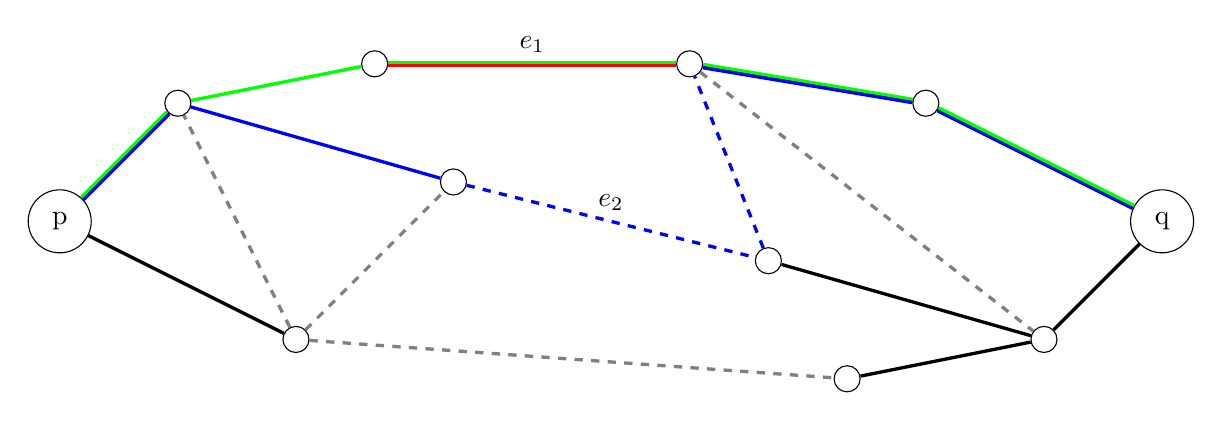
\begin{tikzpicture}
        \begin{scope}[every node/.style={circle,draw}]
            \node[minimum size=0.8cm] (a) at (-7,0) {p};
            \node[minimum size=0.8cm] (b) at (7,0) {q};
            \node (c) at (-5.5,1.5) {};
            \node (d) at (5.5,-1.5) {};
            \node (e) at (-4,-1.5) {};
            \node (f) at (4,1.5) {};
            \node (g) at (-3,2) {};
            \node (h) at (3,-2) {};
            \node (i) at (-2,0.5) {};
            \node (l) at (2,-0.5) {};
            \node (m) at (1,2) {};
        \end{scope}
        \begin{scope}[every edge/.style={very thick,draw}]
            \path [-] (a) edge[side by side=green:blue] (c);
            \path [-] (a) edge (e);
            \path [-] (c) edge[draw=green] (g);
            \path [-] (c) edge[draw=blue] (i);
            \path [-] (b) edge (d);
            \path [-] (d) edge (h);
            \path [-] (d) edge (l);
            \path [-] (b) edge[side by side=blue:green] (f);
            \path [-] (g) edge[side by side=green:red] node[above]{$e_1$} (m);
            \path [-] (m) edge[side by side=green:blue] (f);
        \end{scope}
        \begin{scope}[every edge/.style={very thick,dashed,draw=gray}]
            \path [-] (i) edge[draw=blue] node[above]{$e_2$} (l);
            \path [-] (l) edge[draw=blue] (m);
            \path [-] (e) edge (i);
            \path [-] (e) edge (c);
            \path [-] (e) edge (h);
            \path [-] (m) edge (d);
        \end{scope}
    \end{tikzpicture}
    \caption{In verde: il cammino $\sigma(p,q)$, in blu: il cammino $\mu(p,q)$}
\end{figure}
\begin{proof}
Sia $T$ un MST, e sia $\sigma(p,q)$ un cammino dal nodo $p$ al nodo $q$ in $T$. Supponiamo per assurdo che esista un cammino $\mu(p,q)$ con peso massimo inferiore. Tagliamo $T$ in due frammenti rimuovendo un arco $e_1$ di peso massimo in $\sigma(p,q)$. Da ipotesi, per ogni arco $e$ in $\mu(p,q)$, vale $w(e)<w(e_1)$. Allora, esiste un arco attraversante $e_2$ in $\mu(p,q)$ che produce uno \eng{spanning tree} di peso minore. Ma allora $T$ non era un MST, assurdo. Il cammino nell'MST tra due nodi è sempre un cammino minimax.
\end{proof}
Si nota che possono esistere cammini minimax non contenuti nell'MST, anche nel caso sia unico.

\chapter{Il linguaggio Erlang}

I contenuti di questo capitolo sono tratti dal libro \eng{The BEAM Book}~di~Erik~Stenman~\cite{Stenman_2017}.
\bigskip

\href{https://www.erlang.org/}{Erlang} è un linguaggio funzionale orientato allo sviluppo di software distribuito, con una forte enfasi sulla concorrenza. Per \emph{concorrenza}, si intende la possibilità che più processi vengano eseguiti in maniera non strettamente sequenziale, ma non necessariamente parallela.

\section{Il modello ad attori}
Il modello ad attori è un modello astratto di computazione concorrente introdotto da Carl Hewitt nel 1973~\cite{10.5555/1624775.1624804}. Un \emph{attore} è definito come un'entità di elaborazione con un proprio stato, in grado di comunicare con altri attori esclusivamente attraverso lo scambio di messaggi, in maniera sincrona. Un attore un può inviare un messaggio a un altro attore solamente se ne conosce l'\emph{indirizzo}, e a ogni indirizzo è associato al più un attore (nel caso un attore muoia, l'indirizzo diventa inattivo). Alla ricezione di un messaggio un attore può effettuare le seguenti operazioni:
\begin{itemize}
    \item inviare una quantità finita di messaggi ad altri attori,
    \item creare un numero finito di altri attori,
    \item modificare il proprio stato interno e definire le operazioni da intraprendere alla prossima ricezione di un messaggio
\end{itemize}
Gli indirizzi possono essere ottenuti alla creazione di nuovi attori o tramite messaggio. Il vantaggio principale del modello ad attori è che non necessita di meccanismi di \eng{locking}, dal momento che un attore non può modificare direttamente lo stato interno di un altro attore.

I processi Erlang fungono da attori, seppur imponendo alcuni vincoli aggiuntivi. Ogni processo esegue le proprie istruzioni in maniera sequenziale, la concorrenza è solo tra processi. In aggiunta, i messaggi da un certo mittente vengono ricevuti nello stesso ordine in cui sono stati inviati. Quest'ultimo comportamento può essere simulato nel modello standard aggiungendo un contatore ai messaggi inviati, in modo tale che il destinatario possa riordinarli in una coda FIFO per mittente.

\section{I processi Erlang}

Un processo Erlang è funzionalmente simile a un processo nativo del sistema operativo, nel senso che ha un proprio identificativo ``PID'', il proprio spazio d'indirizzi e può comunicare con altri processi attraverso segnali e messaggi. La differenza cruciale è che in Erlang i processi sono implementati come \eng{thread virtuali} (\emph{\eng{green thread}}) a basso \eng{overhead}, efficienti sia da creare che distruggere.

\subsection{L'architettura \eng{shared-nothing}}

I processi sono isolati secondo l'architettura ``\eng{shared-nothing}'' (SN), dove le situazioni di contesa sono evitate eliminando l'accesso condiviso alle risorse. L'architettura SN porta vantaggi nella scalabilità e resilienza di un sistema poiché i processi possono essere trattati come componenti indipendenti.

\paragraph{Scalabilità}
Dal momento che non c'è una risorsa centrale condivisa, un sistema SN può scalare semplicemente aumentando il numero di processi senza incappare in colli di bottiglia.

\paragraph{\eng{Let it crash}}\label{erl:crash}
In un sistema, si definisce ``\eng{single point of failue}'' un componente il cui malfunzionamento può portare alla compromissione dell'intero sistema. L'architettura SN aiuta a mitigare questo fenomeno, in quanto gli effetti degli errori di programmazione fatali sono confinati al processo in cui il codice erroneo è in esecuzione. Le altre componenti possono decidere semplicemente di riavviare il processo, o intraprendere altre azioni correttive. L'impiego sistematico di questa strategia per gestire gli errori costituisce il design pattern ``\eng{Let it crash}''.

\section{Il sistema \eng{runtime} di Erlang}

Il codice Erlang compilato viene eseguito nell'Erlang \eng{Runtime System}, del quale ``ERTS'' è l'implementazione standard \emph{de facto} distribuita in ``Erlang/OTP''. Originariamente, OTP (\eng{Open Telecom Platform}) era una raccolta di librerie che forniva gli strumenti di base per sviluppare applicazioni distribuite nel campo delle telecomunicazioni, tuttavia al giorno d'oggi è stata in gran parte integrata nelle librerie standard Erlang. Erlang/OTP è ora il nome della distribuzione Erlang standard, che include ERTS, un compilatore e altri strumenti di diagnostica.

\paragraph{I nodi Erlang}
Un sistema distribuito Erlang è costituito da un certo numero di istanze di un \eng{Erlang Runtime System} connesse, ciascuna contenente un numero arbitrario di processi. Quando a un'istanza viene assegnato un nome, prende il nome di ``nodo''. Il nome di un nodo è necessario affinché altri nodi possano comunicare con esso. %Dal momento che tratteremo solo istanze singole, per semplicità chiameremo nodi anche le istanze ERTS senza nome.
\bigskip

ERTS è costituito dalla macchina virtuale BEAM con scheduler, un \eng{kernel} che fornisce servizi di basso livello come la gestione degli I/O e la libreria standard \lstinline{stdlib}.

\subsection{Lo scheduler}

Un'istanza ERTS, nel caso più semplice, consiste in un singolo processo nativo in cui i processi Erlang sono eseguiti in \eng{multitasking}. Lo scheduler mantiene due code: una coda \emph{\eng{ready}} di processi pronti per essere eseguiti e una coda \emph{\eng{waiting}} di processi in attesa di un messaggio. Lo scheduler seleziona il primo processo dalla coda \eng{ready}, e lo passa alla macchina virtuale BEAM che lo esegue per un quanto di tempo. Se il processo non termina entro il quanto di tempo, viene sospeso e lo scheduler lo reinserisce in fondo alla coda \eng{ready}. Se invece il processo si blocca su un'istruzione \lstinline{receive}, viene immediatamente trasferito nella coda \eng{waiting}. Per ragioni di efficienza, un processo può essere sospeso solo al momento di una chiamata a funzione o una \lstinline{receive}.

\paragraph{\eng{Multitasking} con prelazione}
Nonostante i processi siano implementati come thread virtuali, il modello di \eng{multitasking} di Erlang è con prelazione. In genere, questo non è possibile, è necessario che ogni thread virtuale chiami periodicamente una procedura apposita per restituire il controllo del processore allo scheduler (\eng{multitasking} cooperativo). Erlang sfrutta due proprietà fondamentali della propria architettura per mantenere in modo efficiente i benefici del \eng{multitasking} con prelazione pur essendo tecnicamente cooperativo:
\begin{itemize}
    \item Erlang è un linguaggio funzionale, e in quanto tale non possiede un costrutto di iterazione. Ignorando la funzione \lstinline{receive} pre-rilasciata da BEAM, è pressoché impossibile che un processo occupi tempo d'esecuzione senza anche effettuare chiamate a funzione. Formalmente, la chiamata a funzione è una \emph{riduzione}, intesa come un qualsiasi evento che può essere usato per rappresentare il tempo d'esecuzione del processo.
    \item Il codice Erlang è eseguito in una macchina virtuale, quindi non può monopolizzare il processore fisico. Difatti, è BEAM stessa che ha il compito di sospendere i processi, decrementando un contatore a ogni riduzione. Quando il contatore raggiunge lo $0$, la macchina virtuale sospende il processo e lo scheduler ne seleziona un altro.
\end{itemize}
Le funzioni native sono casi speciali dove è necessario il \eng{multitasking} cooperativo esplicito.
\bigskip

Un’istanza ERTS può anche sfruttare più processori, se disponibili, tramite l'utilizzo di thread nativi, ovvero thread gestiti dal sistema operativo. Ogni thread ha una macchina virtuale e scheduler indipendenti. Un sottosistema di bilanciamento del carico mantiene le code di ogni scheduler bilanciate, al costo di dover utilizzare \eng{locks} per evitare \eng{race conditions}.

\subsection{La macchina virtuale BEAM}

BEAM è una macchina virtuale a registri con \eng{garbage collector} che esegue il \eng{bytecode} prodotto dal compilatore. In maniera equivalente ai file \lstinline{.class} Java, il compilatore produce file \lstinline{.beam} di \eng{bytecode} BEAM indipendente dall'architettura nativa. L'esecuzione delle istruzioni BEAM è accelerata utilizzando la tecnica del \emph{\eng{direct threading}}:

\paragraph{Il \eng{direct threading}}
Il \emph{\eng{threading}} è una tecnica dove le istanze di una stessa porzione di codice macchina sono sostituite con un riferimento a un'unica implementazione comune. Il \eng{\emph{direct} threading} è un modello di \eng{threading} dove i riferimenti sono indirizzi al codice dell'implementazione, e ogni implementazione termina direttamente con un salto all'indirizzo successivo.
\bigskip

Nella macchina virtuale BEAM, ogni istruzione nel \eng{bytecode} viene sostituita con l'indirizzo al codice nativo che implementa l'istruzione. Ciò permette di avere una logica di esecuzione sostanzialmente più semplice e performante.

% \subsection{Lo scheduler}

\section{Comunicazione tra processi}

A livello di linguaggio, la comunicazione tra processi Erlang avviene esclusivamente tramite scambio di messaggi. Un messaggio è inviato mediante l'operatore \emph{\eng{send}} \lstinline{Dst ! Msg}, dove il valore di \lstinline{Msg} è il contenuto del messaggio, e il valore di \lstinline{Dst} è un identificativo del destinatario, come ad esempio il PID. Ogni processo possiede una coda di ricezione di messaggi chiamata ``\eng{mailbox}'' a cui si accede con il costrutto \lstinline{receive}. Il messaggio viene cercato nella \eng{mailbox} in ordine di arrivo tramite \emph{pattern \eng{matching}}. Se non esiste un messaggio che soddisfa i pattern forniti, il processo si blocca in attesa del prossimo messaggio.

Internamente a ERTS, l'unico meccanismo di comunicazione tra processi sono i \emph{segnali}. I segnali, a differenza dei messaggi, non contengono dati, ma hanno ognuno un significato prestabilito dall'implementazione. In generale, la maggior parte delle operazioni che coinvolgono più processi sono implementate con i segnali, inclusi i messaggi.

\subsection{Invio di messaggi}

La \eng{mailbox} di un processo è implementata con due code: la coda \lstinline{signal} e la coda \lstinline{message}. Quando si invia un messaggio, se ne crea una copia e si aggiunge un riferimento nella coda \lstinline{signal} del destinatario. La copia semplifica la procedura di \eng{garbage collection}, poiché in questo modo i messaggi ricevuti sono in zone di memoria indipendenti dai processi che li hanno inviati. 

Di default, la copia avviene direttamente nella \eng{heap} del destinatario. Questo approccio è sufficiente solo nel caso tutti i processi siano eseguiti in \eng{multitasking} su un singolo scheduler, senza possibilità di \eng{race coditions}. In generale, quest'operazione richiede il possesso di un lock su tutta la \eng{heap} del destinatario, con latenze non trascurabili.

Qualora non venga ottenuto il lock, il messaggio viene copiato in una nuova zona di memoria chiamata \emph{\eng{heap fragment}}. È comunque necessario acquisire un lock sulla coda \lstinline{signal}, ma l'aggiunta del riferimento è immediata. Il costo dell'allocazione dell'\eng{heap fragment} invece non dipende dalla quantità di messaggi in arrivo. 

\subsection{Ricezione di messaggi}

I messaggi nella coda \lstinline{signal} sono spostati periodicamente nella coda \lstinline{message} automaticamente. La ricerca del messaggio è effettuata esclusivamente nella coda \lstinline{message} per prevenire situazioni di contesa con i processi in fase di invio.

In Erlang, i pattern possono contenere variabili \eng{bounded}; ciò comporta che a ogni \lstinline{receive} è necessario ripetere la ricerca partendo dall'inizio della coda \lstinline{message}. Potrebbe succedere che nella coda si accumulino un gran numero di messaggi che non soddisfano nessun pattern, penalizzando le prestazioni. Questo fenomeno è intrinseco al design del costrutto e non può essere eliminato completamente.

Per mitigare il costo della ricerca, in alcune situazioni Erlang impiega un'ottimizzazione che sfrutta la creazione di valori globalmente unici per saltare il controllo di un certo numero di messaggi. Ad esempio, se un pattern contiene una variabile che nello \eng{scope} corrente è stata inizializzata con la funzione \lstinline{spawn} (la primitiva per creare processi), i messaggi precedenti vengano ignorati, poiché il PID di un processo è unico. In ogni caso, il consumo di memoria della coda aumenta.
\bigskip

Quando i processi sono in esecuzione in nodi Erlang diversi, lo scambio di messaggi avviene in maniera trasparente. Tuttavia, c'è il rischio che i messaggi vengano persi durante il trasporto. La ricezione dei messaggi è garantita finché esiste una connessione affidabile tra i nodi. Erlang include degli strumenti per monitorare lo stato di un processo sia locale che remoto, ma non possono garantire da soli la tolleranza del sistema alle partizioni della rete.

In generale, per il CAP~\eng{theorem}~\cite{10.1145/564585.564601}, un sistema distribuito non può essere contemporaneamente consistente, disponibile e tollerante alle partizioni. Erlang non impone nessuna delle tre proprietà, quindi sviluppando un sistema si può scegliere quali garantire.

\chapter{Implementazione}

L'algoritmo è stato implementato sotto forma di una demo scritta in Erlang e un validatore scritto in Python. La demo genera un grafo~Kronecker~stocastico~\ref{impl:kronecker}, con numero di nodi passato come argomento, e avvia un processo per ogni nodo, collezionandone i PID. A ogni nodo vengono inviate le informazioni sui vicini sotto forma di una lista di nodo adiacenti, in cui ogni elemento contiene il peso dell'arco e il PID del processo corrispondente, dopodiché a ogni nodo viene inviato un messaggio \lstinline{start} e l'algoritmo comincia.

Alla terminazione, l'\eng{output} viene scritto su \lstinline{stdout} in formato json e opzionalmente passato al validatore. Il validatore confronta i risultati della demo con i risultati ottenuti sullo stesso grafo dalla libreria \eng{peer-reviewed} di manipolazione di grafi \href{https://networkx.org/}{NetworkX}~\ref{impl:verify}.

\section{Scelta del tipo di implementazione}

In genere, l'implementazione di un algoritmo è resa disponibile in forma di libreria o modulo, in modo tale che altri programmi possano farne uso. Erlang è dotato nativamente di un sistema di moduli; tuttavia il costrutto \lstinline{receive}, così come è definito, può limitarne l'utilità in implementazioni specifiche:
\begin{lstlisting}[language=Erlang]
receive
   pattern1 ->
       actions1;
   pattern2 ->
       actions2;
   ....
   patternN
       actionsN
end.
\end{lstlisting}
Il costrutto \lstinline{receive} non supporta l'unione, ovvero i pattern di più \lstinline{receive} non possono essere ``fusi'' in un'unica selezione. I pattern dell'algoritmo GHS devono essere scritti esplicitamente nella \eng{receive} primaria del programma. Il costrutto \lstinline{receive} non supporta nemmeno l'annidamento, in quanto il match di un pattern rimuove un messaggio dalla \eng{mailbox}.

Una prima possibile soluzione a questo problema sarebbe aggiungere nella \lstinline{receive} primaria un match di default, e passare il messaggio a una funzione di \eng{handling} importata dal modulo. Per gestire lo stato, la funzione dovrebbe restituire un opportuno tipo monadico. In questo modo diventa semplice comporre funzioni di \eng{handling} importate da vari moduli nella propria \lstinline{receive} a patto che utilizzino la stessa monade. Erlang non supporta nativamente le monadi, quindi quest'opzione potrebbe essere poco praticabile.

Una seconda soluzione sarebbe racchiudere completamente la logica dell'algoritmo dentro un'unica funzione esportata. Questa opzione ha il difetto che la logica del programma rimarrebbe bloccata finché l'algoritmo non ha terminato~\ref{impl:termination}. Lo stato finale del nodo verrebbe restituito dalla funzione.

\section{Grafi generati mediante prodotto di Kronecker}\label{impl:kronecker}

Il prodotto Kronecker è una specializzazione del prodotto tensoriale su matrici di dimensione arbitraria risultante in una matrice di dimensioni maggiori. Date due matrici $A\in\mathbb{R}^{m\times n}$ e $B\in\mathbb{R}^{k\times l}$, il prodotto Kronecker $A\otimes B$ è una matrice $\mathbb{R}^{nk\times ml}$:
$$
A\otimes B=\begin{pmatrix}
  a_{11}B & \cdots & a_{1n}B\\
  \vdots & \ddots & \vdots\\
  a_{m1}B & \cdots & a_{mn}B 
\end{pmatrix}
$$
I grafi Kronecker utilizzano iterativamente il prodotto Kronecker per costruire una matrice di adiacenza di dimensione arbitraria $G_k$ partendo dalla matrice di un piccolo grafo generatore $G_1$:
$$
G_k\:=\:\underbrace{G_1\otimes G_1\otimes\:\ldots\: G_1}_{k\text{ iterazioni}}
$$
I grafi Kronecker \emph{stocastici} sono generati da una matrice di adiacenza probabilistica dove ogni valore indica la probabilità che esista l'arco.

I grafi Kronecker sono ottimi candidati per generare reti sociali artificiali~\cite{10.5555/1756006.1756039}, poiché presentano molte caratteristiche tipiche delle reti sociali reali, come la distribuzione \eng{power-law} dei gradi e il diametro piccolo (effetto \eng{small word}).

Il grafo nella demo è generato partendo da una matrice $2\times 2$, che nel nostro caso ha la seguente forma:
$$
\begin{pmatrix}
  0,99 & 0,54 \\
  0,54 & 0,13
\end{pmatrix}
$$
Questa matrice è derivata dai risultati in \cite{10.5555/1756006.1756039}, dove è stato utilizzato l'algoritmo di \eng{fitting} KronFit per modellare la rete sociale del sito di recensioni ``\eng{Epinions}''. È stata leggermente alterata per ottenere una matrice diagonale.

Il prodotto viene iterato $\lceil{\log_2{n}}\rceil-1$ volte, dove $n\geq 2$ è il numero desiderato di nodi. Se $n$ non è una potenza di $2$ viene semplicemente utilizzata una porzione $1,\dotsc,n$ della matrice. Si nota che se la matrice generatrice è simmetrica, lo sarà anche la matrice risultante. Questa proprietà è utile quando si vogliono modellare grafi non orientati.

Nel nostro caso, a ogni valore $g_{ij}$ nella matrice Kronecker $G_k$ viene applicata la correzione $(1-g_{ij})^2$, e otteniamo grafi casuali quasi completi.
\begin{figure}[H]
    \centering
    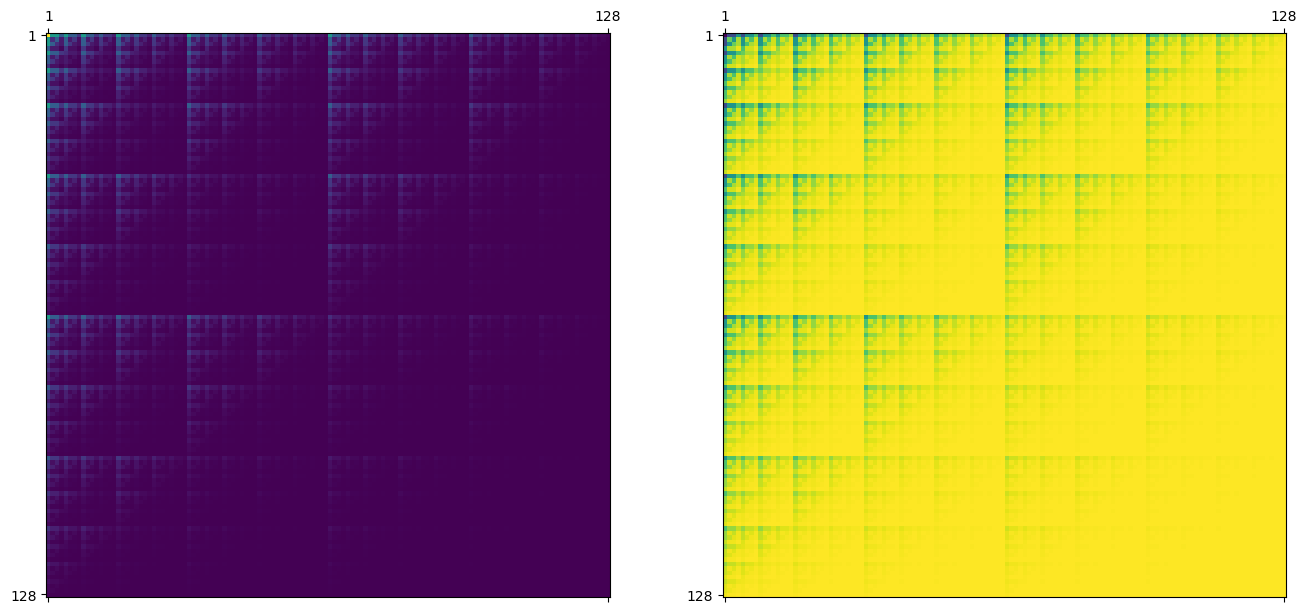
\includegraphics[width=1\linewidth]{images/kronecker-adjacency.png}
    \caption{A sinistra: il risultato di $7$ iterazioni del prodotto Kronecker. A destra: la matrice corretta}
    \label{fig:enter-label}
\end{figure}

\section{Validazione}

\subsection{Riconoscere la terminazione}\label{impl:termination}

Come menzionato nella sezione ``Algoritmi distribuiti''~\ref{algs:distributed}, un algoritmo distribuito termina quando raggiunge una configurazione in cui, globalmente, nessun passo di computazione è applicabile. Questa definizione è simile alla definizione di terminazione di un generico modello di calcolo non distribuito, dove essendoci un singolo esecutore il cui stato è noto, è facile decidere che l'algoritmo è concluso. In un sistema distribuito la configurazione globale non è nota ai singoli nodi, quindi non è detto che ogni nodo possa decidere autonomamente la terminazione. Con gli algoritmi di leader \eng{election} e \eng{rieliable broadcast} è possibile decidere e propagare lo stato di terminazione a patto che tutti i nodi siano raggiungibili tra loro.

Al fine di poter validare i risultati del'implementazione, il programma deve terminare con dei risultati. L'algoritmo GHS risolve i problemi leader \eng{election}~\ref{ghs:election} e \eng{reliable broacast}~\ref{ghs:broadcast}, tuttavia in questa demo viene applicato a grafi non necessariamente connessi. Non potendo prevedere il numero finale di leader di cui attendere la terminazione, è stato introdotto un nodo ausiliario connesso a tutti i nodi che decide la terminazione. Questo nodo ``supervisore'' non è parte dell'algoritmo, e non è realistico poiché se esistesse, sarebbe già un leader connesso direttamente a ogni nodo.

Il processo supervisore mantiene un contatore del numero totale di nodi nel grafo. Ogni volta che riceve un messaggio \msg{done} da uno dei nodi, decrementa il contatore. Quando il contatore scende a $0$, il supervisore chiama una funzione conclusiva, invia a tutti i nodi un messaggio \msg{die} e termina. Alla ricezione del messaggio \msg{die} i nodi terminano, e alla terminazione dell'ultimo processo il \eng{runtime} si chiude. Questo approccio richiede che si conosca a priori il numero totale di nodi (chiamato anche un approccio non uniforme), un'alternativa è fare in modo che i nuovi processi si annuncino al supervisore affinché incrementi il contatore.

\subsection{Verifica dei risultati}\label{impl:verify}

La strategia di validazione dei risultati che si è scelta è il confronto dei pesi degli MST calcolati dall'algoritmo con i pesi degli MST calcolati dalla libreria NetworkX. A tal scopo è stato necessario implementare in Erlang una procedura distribuita per il calcolo del peso dell'albero, e definire un rappresentante degli MST per identificarli nel confronto.

Alla conclusione dell'algoritmo GHS si ottiene un \eng{sink tree} diretto verso il nodo core, il leader della componente connessa. In ogni componente, il core è l'unico nodo in grado di decidere il completamento dell'algoritmo, poiché avvia l'ultima \eng{search} e riceve in \eng{convergecast} \msg{report}[$\infty$]. Il calcolo della dimensione dell'MST avviene subito dopo, con un semplice \eng{broadcast} e \eng{convergecast} attraverso il \eng{sink tree}. Il leader invia un messaggio \msg{broadcast} che viene propagato da ogni nodo verso i figli; una volta raggiunte le foglie, inizia il \eng{convergecast} verso il leader dove il peso di ogni arco viene sommato. Quando il leader riceve il totale, lo comunica al supervisore.

\paragraph{Scelta del rappresentante}
Istintivamente, si potrebbe pensare di scegliere semplicemente il nodo core come rappresentante dell'albero, tuttavia GHS lo sceglie in modo praticamente casuale e non deterministico. Il validatore dovrebbe determinare quale core appartiene a ciascuno degli MST ottenuti con il proprio algoritmo (in più, in caso di errore, potrebbe ottenere più MST che core). Per semplificare al massimo il codice di validazione, si è deciso di sfruttare il \eng{convergecast} e scegliere il nodo con PID massimo come rappresentante.
\bigskip

Ogni volta che un nodo propaga l'informazione verso il genitore, invia anche il messaggio \msg{done} al supervisore per segnalare che è pronto per la terminazione. La demo termina stampando su \lstinline{stdout} una serializzazione json del grafo e un vettore di coppie rappresentante - peso.
\bigskip

Una strategia di validazione alternativa, più rigorosa, è verificare l'isomorfismo di ogni MST. Conviene comunque definire un rappresentante per stesse ragioni precedentemente espresse, un altro requisito aggiuntivo è che lo stesso criterio di disambiguazione degli archi va replicato nel validatore~\ref{ghs:weights}. Determinare se due alberi (grafi non orientati connessi e aciclici) sono isomorfismo ha complessità lineare sulla dimensione dell'albero~\cite{10.5555/578775}. La rappresentazione completa dell'MST può essere ottenuta sempre per via di un \eng{broadcast}. La libreria NetworkX offre un algoritmo di calcolo dell'isomorfismo tra alberi con complessità $O(n\log n)$.

\section{Calcolo dei cammini minimax distribuito}

Come si è visto, un algoritmo per il calcolo degli MST può essere usato per risolvere anche il problema del cammino minimax~\ref{ghs:minimax}. Il calcolo del cammino minimax è stato implementato associando a ogni nodo una tabella di instradamento contenente una voce \eng{\emph{next-hop}} per ogni nodo discendente. Alla ricezione di un messaggio \msg{route}[$Dst$, $Msg$] non destinato al nodo corrente, se il destinatario è presente nella tabella lo si inoltra al \eng{next-hop}, altrimenti lo si inoltra al genitore (in modo simile a un \eng{\emph{default gateway}}). Si ricorda che tra due nodi in un albero esiste sempre un unico cammino\ref{mst:path}, e in un albero con radice passa per l'antenato comune più stretto. La tabella del nodo core \,\textendash\,~la radice dello \eng{spanning tree}~\,\textendash\, ha una voce per ogni nodo dell'albero. In alcuni contesti reali, questo approccio \eng{naive} potrebbe portare ad avere tabelle di instradamento di dimensioni proibitive. Questo è un problema comunemente risolto con metodi di compressione delle voci, ad esempio mediante i \eng{prefix tree}.

Le tabelle sono popolate sfruttando lo stesso \eng{broadcast} per il calcolo del peso dell'albero.

\section{Struttura del progetto}

OTP definisce delle linee guida su come strutturare un progetto Erlang per garantire la compatibilità con gli strumenti di sviluppo come gestori delle dipendenze, \eng{build systems} o \href{https://hex.pm/}{\eng{repository} di pacchetti}. In generale, i progetti possono essere distinti tra ``applicazioni'' e ``release'':
\begin{itemize}
    \item Un'applicazione è un progetto concepito per essere utilizzato in altri progetti. La categoria comprende sia applicazioni eseguibili che librerie, intese come raccolte di moduli. Le applicazioni eseguibili contengono un file manifesto ``\eng{application resource file}'' che definisce come devono essere gestite dal processo \eng{built-in} ``\eng{application controller}'', con il quale il programmatore interagisce. Un esempio di applicazioni sono il \eng{kernel} e in generale le librerie incluse in Erlang/OTP.
    \item Una ``release'' è un pacchetto composto dal \eng{runtime} ERTS, una collezione di applicazioni e un sottoinsieme di applicazioni Erlang/OTP. In altre parole è un'intera distribuzione Erlang autosufficiente, contenente solo gli elementi necessari a eseguire un set di applicazioni scelte dal programmatore. La distribuzione Erlang/OTP è essa stessa una release, contenente tutte e sole le applicazioni Erlang/OTP. Le release possono essere distribuite come binari o container. Un'istanza di una release costituisce a tutti gli effetti un nodo Erlang.
\end{itemize}
Le linee guida OTP sono fortemente orientate verso lo sviluppo di sistemi scalabili e tolleranti ai guasti, e prevedono che le applicazioni seguano il design pattern ``\eng{supervisor tree}'' basato sulla filosofia ``\eng{let it crash}'' tipica di Erlang~\ref{erl:crash}. Tuttavia, esse risultano completamente inadeguate allo sviluppo di applicazioni ``tradizionali'' con un singolo \eng{entry point}, come ad esempio gli strumenti CLI.

\paragraph{Gli script Erlang}
Con ERTS è incluso l'interprete di script Erlang \lstinline{escript}. Gli script esportano una funzione \lstinline{main(Args)} che l'interprete invoca su una lista di stringhe rappresentanti gli argomenti. Opzionalmente, si può precompilare lo script per ottenere prestazioni migliori, infatti uno script non dev'essere per forza un file di testo, può anche contenere un file \lstinline{.beam} o un archivio. Gli script Erlang sono ideali per implementare piccole applicazioni semplici, quindi la demo è stata implementata in questo formato.
\bigskip

La demo è compilata utilizzando \href{https://rebar3.org/}{Rebar3}, il \eng{build system} ufficiale di Erlang. \eng{Rebar3} è costruito sopra le linee guida OTP, offre un potente sistema di \eng{plugin} ed è usato come backend dalla maggior parte degli strumenti di sviluppo, come i \eng{language server} e i \eng{code formatter}.
\bigskip

La \eng{repository} con i sorgenti della demo è disponibile online al seguente \href{https://github.com/Lucide/Gallager-Humblet-Spira}{link}.

%% Fine dei capitoli normali, inizio dei capitoli-appendice (opzionali)
\appendix

%\part{Appendici}

%\chapter{Titolo della prima appendice}

%% Parte conclusiva del documento; tipicamente per riassunto, bibliografia e/o indice analitico.
\backmatter

%% Riassunto (opzionale)
%\summary


%% Bibliografia (praticamente obbligatoria)
\bibliographystyle{plain_\languagename}%% Carica l'omonimo file .bst, dove \languagename è la lingua attiva.
%% Nel caso in cui si usi un file .bib (consigliato)
\bibliography{thud}
%% Nel caso di bibliografia manuale, usare l'environment thebibliography.

%% Per l'indice analitico, usare il pacchetto makeidx (o analogo).

\end{document}

--- Istruzioni per l'aggiunta di nuove lingue ---
Per ogni nuova lingua utilizzata aggiungere nel preambolo il seguente spezzone:
    \addto\captionsitalian{%
        \def\abstractname{Sommario}%
        \def\acknowledgementsname{Ringraziamenti}%
        \def\authorcontactsname{Contatti dell'autore}%
        \def\candidatename{Candidato}%
        \def\chairname{Direttore}%
        \def\conclusionsname{Conclusioni}%
        \def\cosupervisorname{Co-relatore}%
        \def\cosupervisorsname{Co-relatori}%
        \def\cyclename{Ciclo}%
        \def\datename{Anno accademico}%
        \def\indexname{Indice analitico}%
        \def\institutecontactsname{Contatti dell'Istituto}%
        \def\introductionname{Introduzione}%
        \def\prefacename{Prefazione}%
        \def\reviewername{Controrelatore}%
        \def\reviewersname{Controrelatori}%
        %% Anno accademico
        \def\shortdatename{A.A.}%
        \def\summaryname{Riassunto}%
        \def\supervisorname{Relatore}%
        \def\supervisorsname{Relatori}%
        \def\thesisname{Tesi di \expandafter\ifcase\csname thud@target\endcsname Laurea\or Laurea Magistrale\or Dottorato\fi}%
        \def\tutorname{Tutor aziendale%
        \def\tutorsname{Tutor aziendali}%
    }
sostituendo a "italian" (nella 1a riga) il nome della lingua e traducendo le varie voci.
